% Technical note: NuMI target and NOvA detector geometry, distances and neutrino time of flight.
% Numbers in the tables are generated from reports/nova.json by scripts/make_note_tables.py.
\documentclass[11pt,letterpaper]{article}
\usepackage[margin=1in]{geometry}
\usepackage{amsmath,amssymb}
\usepackage{booktabs}
\usepackage{graphicx}
\usepackage{siunitx}
\usepackage{textcomp}
\usepackage{array}
\usepackage{longtable}
\usepackage{microtype}
\usepackage[numbers,sort&compress]{natbib}
\usepackage[hidelinks]{hyperref}
\usepackage{xcolor}
\sisetup{group-separator={,},group-minimum-digits=4,group-digits=integer,detect-weight=true,mode=text}
\graphicspath{{figures/}}
\newcommand{\gpstofversion}{0.7.0}\newcommand{\reportgenerated}{2026-11-06}

\newcommand{\ND}{ND}
\newcommand{\FD}{FD}
\newcommand{\tick}{tick}
\newcommand{\code}[1]{\texttt{#1}}
\setlength{\parskip}{3pt}

\title{\bfseries Determination of the Neutrino Time of Flight from the NuMI Target to the NOvA Detectors:\\[3pt] Coordinate Systems, Distances and Timing Offsets\\[6pt] \normalsize NOvA internal note NOvA-doc-XXXX}
\author{A.~Norman\\ \small Fermi National Accelerator Laboratory}
\date{\today\\ \small gps-tof version \gpstofversion; report generated \reportgenerated}

\begin{document}
\maketitle

\begin{abstract}
This note derives, in full, the straight-line distances between the NuMI target, the NOvA Near Detector (\ND), the NOvA Far Detector (\FD) at Ash River and the MINOS Far Detector at Soudan, and the corresponding neutrino times of flight in SI units and in \SI{64}{MHz} NOvA clock ticks.  Five coordinate systems are used and written out explicitly: a spherical Earth, WGS84 geodetic coordinates and the Earth-centred Earth-fixed (ECEF) frame, the Fermilab Site Coordinate System (a double stereographic projection), the NuMI beamline system with origin MCZERO in which the Fermilab alignment group surveyed both NOvA upstream-face centres, and a beam-axis frame used for off-axis and opening angles.  The target is taken from the 1998 NuMI Technical Design Report beam sheet; the detector endpoints are the surveyed face centres.  Two further sites, points \SI{100}{ft} below the surfaces of Lake Vermilion and of Lake Superior at Two Harbors, are carried through the same chain.  Every correction between the reference model and the final result is tabulated, together with chord geometry, the Main Injector timing shift, the trigger window, relativistic and instrumental terms, sensitivities and an error budget.  The headline result is a flight time from the \ND{} face to the \FD{} face of \SI{2700.250552}{\micro s}, i.e.\ \num{172816.035} ticks, and a total offset including the 141-turn Main Injector shift of \num{272736} ticks.  The 2013 Mathematica notebook and the 2014 note \cite{norman2014} are reproduced to $10^{-9}$ and their superseded geometries are compared with the surveyed result in an appendix.  All computations are performed by the \code{gps-tof} package \cite{gpstof}; the tables of this note are generated from its JSON report.
\end{abstract}

\tableofcontents

\section{Introduction}
The NOvA data acquisition issues a ``beam'' trigger from the NuMI spill time $t_0$ delayed by the neutrino flight time $t_{\rm delay}$ from the beam source to the far detector.  The spill is nominally \SI{10}{\micro s} long; the DAQ discretises data into \SI{50}{\micro s} microslices and the event builder extracts whole microslices, so the trigger window is the half-open interval \cite{norman2014}
\begin{equation}
\Delta T_{\rm trig} = \left[\, t_0 + t_{\rm delay} - \SI{20}{\micro s},\; t_0 + t_{\rm delay} + \SI{30}{\micro s}\,\right),
\label{eq:window}
\end{equation}
which always overlaps exactly two closed microslices.  $t_{\rm delay}$ has to be set a priori from the geometry.

The 2013 Mathematica notebook \cite{norman2013nb} computed the chord between the MINOS surface-building GPS antenna, lowered by \SI{300}{m}, and an Ash River antenna.  The 2014 note NOvA-doc-11860 \cite{norman2014} documented the antenna fixes and specified antenna-to-detector offsets.  Neither contained the NuMI target, and the horizontal antenna-to-detector vectors were left to be determined.  This note (i) derives the target position from the NuMI Technical Design Report \cite{numitdr1998} through the Fermilab site projection \cite{oshinowo1997}, (ii) records the surveyed upstream-face centres of both NOvA detectors \cite{bocean2026nd,bocean2026fd} in the NuMI beamline system and converts them to geodetic and ECEF coordinates, (iii) writes out every coordinate transformation used, and (iv) tabulates the distances, flight times, angles and uncertainties.  Figures~\ref{fig:plan}--\ref{fig:face} are schematic views of the geometry.

\section{Reference frames and transformations}
\subsection{Angles}
Survey records give angles in sexagesimal form.  Degrees, minutes and seconds are converted to radians by
\begin{equation}
\mathrm{LC}(d,m,s)=\frac{\pi}{180}\left(d+\frac{m+s/60}{60}\right),
\end{equation}
with the hemisphere letter supplying the sign.  Longitudes are east-positive throughout; the 2013 notebook entered west longitudes as positive numbers, which leaves distances unchanged (a reflection is an isometry) but flips the sign of rotation-dependent terms such as the Sagnac correction (Sec.~\ref{sec:effects}).

\subsection{Geodetic coordinates and the ECEF frame}
The reference ellipsoid is WGS84 \cite{wgs84}, with semi-major axis $a$, semi-minor axis $b=a(1-f)$ and first eccentricity $e^2=(a^2-b^2)/a^2$:
\begin{equation}
\begin{aligned}
a&=\SI{6378137}{m}, & 1/f&=298.257223563,\\
b&=\SI{6356752.31424518}{m}, & e^2&=\num{6.69437999e-3}.
\end{aligned}
\end{equation}
The Fermilab site survey is in NAD83 on the GRS80 ellipsoid ($1/f=298.257222101$), which differs from WGS84 by \SI{0.1}{mm} in $b$; the two are treated as coincident, as the Fermilab coordinate-system document itself does \cite{oshinowo1997}.  A point with geodetic latitude $\varphi$, longitude $\lambda$ and ellipsoidal height $h$ maps to Earth-centred Earth-fixed Cartesian coordinates by
\begin{equation}
N(\varphi)=\frac{a}{\sqrt{1-e^2\sin^2\varphi}},\qquad
\begin{aligned}
X&=(N+h)\cos\varphi\cos\lambda,\\
Y&=(N+h)\cos\varphi\sin\lambda,\\
Z&=\bigl(N(1-e^2)+h\bigr)\sin\varphi .
\end{aligned}
\label{eq:ecef}
\end{equation}
$N$ is the prime-vertical radius of curvature.  The $X$ axis passes through the intersection of the equator and the prime meridian, $Z$ through the pole.  The inverse transformation is evaluated iteratively to $10^{-14}$\,rad.  The height $h$ in Eq.~\eqref{eq:ecef} is the height above the ellipsoid.  A GPS receiver's \code{\$GPGGA} altitude is orthometric (above mean sea level), $H$; the same sentence gives the geoid separation $N_g$ and $h=H+N_g$.  Each input position in this note carries an explicit datum, and the conversion appears as a line in the correction ledger.

\subsection{Spherical-Earth model}
As a reference model, used only to show the size of the ellipsoidal correction, the Earth is taken as a sphere of radius $R=a$ and
\begin{equation}
\vec r=(R+h)\,(\cos\varphi\cos\lambda,\;\cos\varphi\sin\lambda,\;\sin\varphi).
\label{eq:sphere}
\end{equation}
A sphere of equatorial radius places both sites about \SI{10}{km} too far from the Earth's centre, and since the chord scales with the radius the Fermilab--Ash River chord comes out \SI{823}{m} (\num{176} ticks) too long (Sec.~\ref{sec:models}).

\subsection{Local frame and antenna-to-detector offsets}
At a point $(\varphi,\lambda)$ the local East, North and Up unit vectors in ECEF are
\begin{equation}
\begin{aligned}
\hat E&=(-\sin\lambda,\;\cos\lambda,\;0),\\
\hat N&=(-\sin\varphi\cos\lambda,\;-\sin\varphi\sin\lambda,\;\cos\varphi),\\
\hat U&=(\cos\varphi\cos\lambda,\;\cos\varphi\sin\lambda,\;\sin\varphi).
\end{aligned}
\label{eq:enu}
\end{equation}
A displacement $(d_E,d_N,d_U)$ from a surveyed point (an antenna) to the physics endpoint (a detector face) is added as $\delta\vec p=d_E\hat E+d_N\hat N+d_U\hat U$.  With the ellipsoid normal as $\hat U$ a purely vertical offset is identical to changing $h$ by $d_U$.  The 2014 note describes the plane tangent to a \emph{sphere}, $\hat U=\vec p/|\vec p|$, which differs from the geodetic normal by the geodetic--geocentric latitude difference (\SI{0.19}{\degree} at these sites); both are implemented and the difference is reported as a sensitivity.

\subsection{Fermilab Site Coordinate System}
\label{sec:fscs}
Beam elements in the NuMI Technical Design Report are given in the Fermilab site system, historically ``DUSAF'' coordinates: $x$ east, $y$ north, $z$ elevation, in US survey feet ($\SI{1}{ft}=1200/3937$~m).  Beams-doc-1148 \cite{oshinowo1997} defines the modern realisation, the FSCS, as a double stereographic projection of NAD83/GRS80 geodetic coordinates: the ellipsoid is mapped conformally to a sphere and the sphere projected stereographically to the plane.  This is the Oblique Stereographic projection, EPSG method 9809 \cite{epsg7-2}.  The defining parameters are listed in Table~\ref{tab:fscs}.

\begin{table}[htbp]\centering\small
\caption{Parameters of the Fermilab Site Coordinate System \cite{oshinowo1997}.}
\label{tab:fscs}
\begin{tabular}{ll}
\toprule
origin (monument A0) latitude $\varphi_0$ & N \ang{41;50;14.312704} \\
origin longitude $\lambda_0$ & W \ang{88;15;41.143123} \\
origin ellipsoidal height $h_0$ & \SI{186.49880}{m} \\
geodetic azimuth of the $+Y$ axis at A0, $\alpha$ & \ang{38;16;48.01429} \\
false easting, false northing & \SI{100000}{ft}, \SI{100000}{ft} \\
scale factor at A0, 720 ft above the DUSAF datum, $F_0$ & 1.000029251309483 \\
DUSAF $\to$ NAVD88 height correction, $\delta H$ & \SI{-0.17308}{m} \\
geoid height at A0 (GEOID93), $N_0$ & \SI{-32.78456}{m} \\
ellipsoid & GRS80 ($a=\SI{6378137}{m}$, $1/f=298.257222101$) \\
\bottomrule
\end{tabular}
\end{table}

With $e$ the first eccentricity and $\varphi_0,\lambda_0$ the origin, the projection constants are
\begin{equation}
\begin{aligned}
\rho_0&=\frac{a(1-e^2)}{(1-e^2\sin^2\varphi_0)^{3/2}},\qquad \nu_0=\frac{a}{\sqrt{1-e^2\sin^2\varphi_0}},\qquad R=\sqrt{\rho_0\nu_0},\\
n&=\sqrt{1+\frac{e^2\cos^4\varphi_0}{1-e^2}},\qquad
w_1=\left[\frac{1+\sin\varphi_0}{1-\sin\varphi_0}\left(\frac{1-e\sin\varphi_0}{1+e\sin\varphi_0}\right)^{e}\right]^{n},\qquad
\sin\chi_0'=\frac{w_1-1}{w_1+1},\\
c&=\frac{(n+\sin\varphi_0)(1-\sin\chi_0')}{(n-\sin\varphi_0)(1+\sin\chi_0')},\qquad w_2=c\,w_1,\qquad \chi_0=\arcsin\frac{w_2-1}{w_2+1},
\end{aligned}
\end{equation}
and a point $(\varphi,\lambda)$ projects to the conformal sphere and then to the plane by
\begin{equation}
\begin{aligned}
\Lambda&=n(\lambda-\lambda_0)+\lambda_0,\qquad
w=c\left[\frac{1+\sin\varphi}{1-\sin\varphi}\left(\frac{1-e\sin\varphi}{1+e\sin\varphi}\right)^{e}\right]^{n},\qquad
\chi=\arcsin\frac{w-1}{w+1},\\
B&=1+\sin\chi\sin\chi_0+\cos\chi\cos\chi_0\cos(\Lambda-\lambda_0),\\
E&=\frac{2R\cos\chi\sin(\Lambda-\lambda_0)}{B},\qquad
N=\frac{2R\,[\sin\chi\cos\chi_0-\cos\chi\sin\chi_0\cos(\Lambda-\lambda_0)]}{B}.
\end{aligned}
\label{eq:stereo}
\end{equation}
The FSCS axes are rotated so that $+Y$ points along the geodetic azimuth $\alpha$, rescaled to true scale at 720 ft above the DUSAF datum, and offset by the false coordinates:
\begin{equation}
X_{\rm FSCS}=\frac{F_0\,(E\cos\alpha-N\sin\alpha)}{\SI{1}{ft}}+\SI{100000}{ft},\qquad
Y_{\rm FSCS}=\frac{F_0\,(N\cos\alpha+E\sin\alpha)}{\SI{1}{ft}}+\SI{100000}{ft}.
\label{eq:fscsrot}
\end{equation}
Heights relate as $h=H_{\rm DUSAF}+\delta H+N_g$ with $N_g$ taken as the A0 value across the site (the GEOID93 slope between A0 and the Main Injector centroid is \SI{1.3}{cm}).  The inverse of Eq.~\eqref{eq:stereo} is the EPSG inverse (iteration on the isometric latitude); the implementation reproduces the EPSG worked example (Amersfoort) to \SI{2}{mm} and the CFMI control point of Beams-doc-1148 to \SI{0.1}{mm} horizontally.  A beam-sheet bearing $\beta$ (degrees counter-clockwise from site East) corresponds to the geodetic azimuth $(90^{\circ}-\beta)+\alpha$ at A0; the NuMI final bearing \ang{152.18332} gives \ang{336.097}, against \ang{336.098} from the 1999 Fermilab--Soudan geodetic survey \cite{bocean1999,soler2000}.

\subsection{NuMI beamline system (origin MCZERO) and the beam-axis frame}
\label{sec:beamline}
The Fermilab alignment group reports NuMI positions in a Cartesian beamline system: origin MCZERO; $X$ positive to beam right (eastward) looking downstream; $Y$ the stationing, positive downstream; $Z$ positive upward and orthogonal to the beam \cite{bocean2026fd,bocean2026nd}.  The same construction serves as the beam-axis frame for off-axis angles.  Given an origin $O$ and a second point $T$ on the line, with ECEF positions $\vec p_O$, $\vec p_T$ and the ellipsoid normal $\hat n_O$ at the origin,
\begin{equation}
\hat u=\frac{\vec p_T-\vec p_O}{|\vec p_T-\vec p_O|},\qquad
\hat h=\frac{\hat u\times\hat n_O}{|\hat u\times\hat n_O|},\qquad
\hat v=\hat h\times\hat u .
\label{eq:frame}
\end{equation}
$\hat u$ is along the line, $\hat h$ to the right looking downstream (horizontal at the origin), $\hat v$ up, orthogonal to the line and in the vertical plane through $\hat n_O$.  A point $P$ with $\vec r=\vec p_P-\vec p_O$ has beamline coordinates and off-axis quantities
\begin{equation}
Y=\vec r\cdot\hat u,\qquad X=\vec r\cdot\hat h,\qquad Z=\vec r\cdot\hat v,\qquad
\theta_{\rm off}=\arctan\frac{\sqrt{X^2+Z^2}}{Y},\qquad
\psi_{\rm clock}=\operatorname{atan2}(X,Z),
\label{eq:offaxis}
\end{equation}
where $\psi_{\rm clock}$ is \ang{0} above the axis and \ang{90} to the right; the inverse is $\vec p_P=\vec p_O+Y\hat u+X\hat h+Z\hat v$.  The angle between a chord $\vec d$ and the axis is $\angle(\vec d,\hat u)$ with components $\operatorname{atan2}(\vec d\cdot\hat h,\vec d\cdot\hat u)$ (right) and $\operatorname{atan2}(\vec d\cdot\hat v,\vec d\cdot\hat u)$ (up).  The opening angle at a vertex $V$ between the chords to $A$ and $B$ is $\angle(\vec p_A-\vec p_V,\vec p_B-\vec p_V)$, decomposed into the azimuth and elevation differences of the two chords at $V$; the transverse distance of $A$ from the line $VB$ is $|\vec p_A-\vec p_V|\sin\angle$.  Angles between vectors are evaluated as $\operatorname{atan2}(|\vec a\times\vec b|,\vec a\cdot\vec b)$ for numerical stability at the microradian level.

\textbf{Realisation for NuMI.}  Two elements of the beamline system are not stated in the survey notes and were established here.  (1) MCZERO lies at the upstream end of horn~1, between the target exit and the horn; it is taken as the horn-1 upstream face of the 1998 TDR beam sheet (row 0089, \SI{1.5}{m} downstream of the target entrance).  The as-built point is not public, so the origin is good to about \SI{1}{m} along the beam, which is \SI{0.2}{ticks} on an \SI{810}{km} chord and nothing transverse.  (2) The direction of the $Y$ axis.  Two candidate lines were tested: the 1998 design axis (target $\to$ decay-pipe end) and the as-built aiming line (MCZERO $\to$ MINOS \FD{} midpoint).  The \FD{} survey note gives an independent NAVD88 elevation of the face centre, $H=\SI{1209.1058}{ft}=\SI{368.535}{m}$, i.e.\ $h\simeq\SI{336.07}{m}$ with the Ash River geoid separation $N_g=\SI{-32.462}{m}$ of the receiver.  The aiming line reproduces it to \SI{+1.5}{m} (\SI{+0.3}{m} with the GEOID18 separation of \SI{-31.221}{m} instead of the receiver's value); the design axis misses it by \SI{17}{m}.  The aiming line is therefore the surveyors' $Y$ axis and is used for both survey points (Sec.~\ref{sec:validation}).

\textbf{Detector faces.}  A face of half-width $w$ and half-height $w'$ centred at $(X,Y,Z)$ has edge points $(X\mp w,Y,Z)$ (left, right) and $(X,Y,Z\pm w')$ (top, bottom) in the same frame; the face is taken perpendicular to the beamline rather than to the detector's own axis, a \SI{3}{cm} difference for the \ND.  The angle the face subtends at the axis origin is $\angle(\vec r_{\rm left},\vec r_{\rm right})$.

\section{Input positions}
\subsection{NuMI target, MCZERO and the design beam axis}
The NuMI Technical Design Report \cite{numitdr1998}, Appendix~A beam sheet ``horn2 ces'', lists every beamline element in DUSAF coordinates (entrance of the device).  The rows used are the target entrance (0087, \code{HALTA TAR-2}), the horn-1 entrance (0089, \code{IHHRN1}, the MCZERO proxy) and the decay-pipe end (0092, \code{DENCU}); the sheet's final bearing is \ang{152.18332} (ccw from site East) and pitch \ang{-3.336}.  These are design positions; as-built target positions in the LE and ME configurations differ at the metre level.

\subsection{Surveyed upstream-face centres of the NOvA detectors}
The definitive endpoints are the upstream-face centres surveyed by the Fermilab Survey, Alignment and Geodesy group \cite{bocean2026nd,bocean2026fd}, Table~\ref{tab:survey}.  The \FD{} point is \SI{7.5}{in} from the intersection of the rail midline with the wall (the bookend) and vertically at the measured highest floor point (\SI{1181.8175}{ft} NAVD88) plus the \SI{23.25}{in} pallet and the \SI{304.21}{in} half-plane, $H=\SI{1209.1058}{ft}$.  The \ND{} point uses the $3\times3$-module width and height of \SI{158.125}{in} and the tunnel cross-section drawing 489389.

\begin{table}[htbp]\centering\small
\caption{Surveyed upstream-face centres in the NuMI beamline system (origin MCZERO; $X$ right, $Y$ stationing, $Z$ up) \cite{bocean2026nd,bocean2026fd}.  Frame as realised in this note.}
\label{tab:survey}
\resizebox{\textwidth}{!}{\begin{tabular}{lrrrl}
\toprule
point & $X$ (m) & $Y$ (m) & $Z$ (m) & frame \\
\midrule
NOvA ND upstream face centre (Fermilab alignment survey) & \num{-11.565000} & \num{993.350283} & \num{-3.643551} & mczero $\rightarrow$ minos-fd \\
NOvA FD upstream face centre (Fermilab alignment survey) & \num{-11037.455993} & \num{810422.323775} & \num{-4162.644422} & mczero $\rightarrow$ minos-fd \\
\bottomrule

\end{tabular}}
\end{table}

\subsection{GPS antenna fixes, MINOS far detector and other inputs}
Table~\ref{tab:inputs} lists the remaining inputs: the MINOS surface-building mast antenna and the three Ash River antennas from the 2014 note \cite{norman2014} (decoded from the TDU receivers' \code{\$GPGGA} sentences; the Table~2 heights of the note are ellipsoidal, as the \code{\$POLYP} altitude confirms), the MINOS \FD{} supermodule midpoint \cite{minos2008} used to define the aiming line, and the 2014-note antenna-derived endpoints that are retained for comparison.

\begin{table}[htbp]\centering\scriptsize
\caption{Other input positions.  FNAL antenna coordinates are quoted to \ang{;;1} (about \SI{31}{m} N--S, \SI{23}{m} E--W); Ash River coordinates to $10^{-6}$ arc-minute.}
\label{tab:inputs}
\begin{tabular}{p{1.5cm}p{3.4cm}p{5.4cm}p{4.3cm}}
\toprule
id & site & position as given & source \\
\midrule
target & NuMI target (TDR 1998) upstream face & FSCS $x,y,z$ = 100327.838, 97780.188, 626.743 ft & NuMI TDR 1998 App. A beam sheet (design); Beams-doc-1148 projection \\
mczero & MCZERO horn 1 upstream face, (TDR 1998) & FSCS $x,y,z$ = 100324.941, 97781.717, 626.552 ft & NuMI TDR 1998 App. A beam sheet row 0089 IHHRN1 \\
decay-end & NuMI decay pipe end (TDR 1998) & FSCS $x,y,z$ = 98230.009, 98887.039, 488.477 ft & NuMI TDR 1998 App. A beam sheet row 0092 DENCU \\
fnal-mast & FNAL MINOS Surface Building mast antenna & 41\textdegree{} 50' 23.0000" N, 88\textdegree{} 16' 13.0000" W, $h$ = \num{228.000} m (ellipsoid) & A.Norman 2014 note Table 2 (MINOS-based TDU receivers) \\
nd-under-mast & ND endpoint if it were under the MINOS mast (105 + 15 m down) & 41\textdegree{} 50' 23.0000" N, 88\textdegree{} 16' 13.0000" W, $h$ = \num{228.000} m (ellipsoid) & 2014 note sec. 3.1 and Tables 2-3 (superseded: the ND is not under the mast) \\
fd1 & Ash River Ant-1 (FD front-face centre) & 48\textdegree{} 22' 42.9468" N, 92\textdegree{} 49' 52.6158" W, $h$ = \num{348.000} m (ellipsoid) & 2014 note Table 2 \\
fd2 & Ash River Ant-2 fix, front face via -19.8 m (antenna-derived, superseded) & 48\textdegree{} 22' 42.9468" N, 92\textdegree{} 49' 52.6158" W, $h$ = \num{348.638} m (ellipsoid) & 2014 note Table 2 (antenna used by the 2013 notebook) \\
fd3 & Ash River Ant-3 (FD front-face centre) & 48\textdegree{} 22' 42.9850" N, 92\textdegree{} 49' 52.6583" W, $h$ = \num{350.346} m (ellipsoid) & 2014 note Table 2 / \$GPGGA 2013-03-07 21:03:41 UTC \\
minos-fd & MINOS Far Detector (supermodule midpoint, Soudan) & 47\textdegree{} 49' 12.9612" N, 92\textdegree{} 14' 29.0832" W, $h$ = \num{-248.400} m (ellipsoid) & MINOS detectors NIM A 596 (2008) 190, sec. 6.5 \\
vermilion & Lake Vermilion (100 ft below the surface) & 47\textdegree{} 50' 49.4300" N, 92\textdegree{} 17' 46.3400" W, $H$ = \num{383.440} m (MSL), $N_g$ = \num{-30.892} m & Coordinates supplied by A. Norman (2026-11-09); surface 1,358 ft (Lake Vermilion, MN DNR / Vermilion Dam); GEOID18 \\
two-harbors & Lake Superior, Two Harbors (100 ft below the surface) & 46\textdegree{} 59' 55.2000" N, 91\textdegree{} 38' 16.6500" W, $H$ = \num{152.735} m (MSL), $N_g$ = \num{-29.103} m & Coordinates supplied by A. Norman (2026-11-09); surface 601.1 ft IGLD85 (NOAA chart datum); GEOID18 \\
\bottomrule

\end{tabular}
\end{table}

\subsection{Lake sites}
\label{sec:lakes}
Two additional points were added at \SI{100}{ft} below the lake surface: Lake Vermilion at \ang{47;50;49.43}\,N, \ang{92;17;46.34}\,W and Lake Superior at Two Harbors, \ang{46;59;55.2}\,N, \ang{91;38;16.65}\,W.  The lake surfaces are \SI{1358}{ft} (Vermilion Dam normal pool, NGVD29) and \SI{601.1}{ft} (Lake Superior chart datum, IGLD~1985), so the points are at orthometric heights $H=\SI{1258}{ft}=\SI{383.440}{m}$ and $H=\SI{501.1}{ft}=\SI{152.735}{m}$.  These are mean-sea-level heights and are converted to ellipsoidal heights with the GEOID18 separations at the two points, $N_g=\SI{-30.892}{m}$ and \SI{-29.103}{m} (NGS geoid service); the conversion is a ledger line (Table~\ref{tab:lakes}).  Lake levels vary by about \SI{\pm 0.6}{m}, worth \SI{0.04}{m} of chord (\SI{0.01}{ticks}), and the NGVD29/IGLD85 to NAVD88 datum differences are at the decimetre level.

\subsection{Converted positions}
Table~\ref{tab:positions} gives every endpoint used below in geodetic (WGS84) and ECEF coordinates after all conversions (site projection, beamline frame, antenna offsets); Table~\ref{tab:positionsdec} repeats the principal points in decimal degrees.

\begin{table}[htbp]\centering\scriptsize
\caption{Endpoints in WGS84 geodetic and ECEF coordinates.  \code{nd}/\code{fd} are the surveyed faces, \code{-left}/\code{-right} their edges; \code{nd-1015}, \code{nd-under-mast} and \code{fd2} are superseded geometries (Appendix~\ref{app:history}).}
\label{tab:positions}
\resizebox{\textwidth}{!}{\begin{tabular}{lllrrrr}
\toprule
id & latitude & longitude & $h$ (m) & $X$ (m) & $Y$ (m) & $Z$ (m) \\
\midrule
target & 41\textdegree{} 49' 55.0917" N & 88\textdegree{} 15' 55.9086" W & \num{158.074} & \num{144061.137} & \num{-4757403.941} & \num{4231821.378} \\
mczero & 41\textdegree{} 49' 55.1213" N & 88\textdegree{} 15' 55.9261" W & \num{158.016} & \num{144060.713} & \num{-4757403.302} & \num{4231822.020} \\
decay-end & 41\textdegree{} 50' 16.5133" N & 88\textdegree{} 16' 08.6061" W & \num{115.930} & \num{143754.011} & \num{-4756940.784} & \num{4232285.708} \\
nd & 41\textdegree{} 50' 24.3467" N & 88\textdegree{} 16' 13.7981" W & \num{96.572} & \num{143628.970} & \num{-4756768.845} & \num{4232452.856} \\
nd-left & 41\textdegree{} 50' 24.3203" N & 88\textdegree{} 16' 13.8777" W & \num{96.572} & \num{143627.151} & \num{-4756769.443} & \num{4232452.250} \\
nd-right & 41\textdegree{} 50' 24.3731" N & 88\textdegree{} 16' 13.7185" W & \num{96.572} & \num{143630.788} & \num{-4756768.247} & \num{4232453.463} \\
fd & 48\textdegree{} 22' 41.5413" N & 92\textdegree{} 49' 50.7737" W & \num{337.611} & \num{-209624.380} & \num{-4239417.585} & \num{4745165.129} \\
fd-left & 48\textdegree{} 22' 41.4272" N & 92\textdegree{} 49' 51.1078" W & \num{337.623} & \num{-209631.378} & \num{-4239419.886} & \num{4745162.796} \\
fd-right & 48\textdegree{} 22' 41.6555" N & 92\textdegree{} 49' 50.4396" W & \num{337.599} & \num{-209617.382} & \num{-4239415.284} & \num{4745167.462} \\
minos-fd & 47\textdegree{} 49' 12.9612" N & 92\textdegree{} 14' 29.0832" W & \num{-248.400} & \num{-167796.989} & \num{-4287098.683} & \num{4703296.906} \\
vermilion & 47\textdegree{} 50' 49.4300" N & 92\textdegree{} 17' 46.3400" W & \num{352.548} & \num{-171824.466} & \num{-4285132.713} & \num{4705742.418} \\
two-harbors & 46\textdegree{} 59' 55.2000" N & 91\textdegree{} 38' 16.6500" W & \num{123.632} & \num{-124565.097} & \num{-4356099.794} & \num{4641754.113} \\
nd-1015 & 41\textdegree{} 50' 24.9725" N & 88\textdegree{} 16' 14.1694" W & \num{104.124} & \num{143620.189} & \num{-4756761.853} & \num{4232472.279} \\
nd-under-mast & 41\textdegree{} 50' 23.0000" N & 88\textdegree{} 16' 13.0000" W & \num{108.000} & \num{143648.469} & \num{-4756804.502} & \num{4232429.524} \\
fd2 & 48\textdegree{} 22' 42.9468" N & 92\textdegree{} 49' 52.6158" W & \num{328.838} & \num{-209660.350} & \num{-4239377.478} & \num{4745187.407} \\
\bottomrule

\end{tabular}}
\end{table}

\begin{table}[htbp]\centering\small
\caption{Principal points in decimal degrees (WGS84).}
\label{tab:positionsdec}
\begin{tabular}{lrrr}
\toprule
id & latitude (\textdegree) & longitude (\textdegree, east +) & $h$ (m) \\
\midrule
target & \num{41.831969923} & \num{-88.265530166} & \num{158.074} \\
mczero & \num{41.831978142} & \num{-88.265535036} & \num{158.016} \\
nd & \num{41.840096298} & \num{-88.270499477} & \num{96.572} \\
fd & \num{48.378205927} & \num{-92.830770475} & \num{337.611} \\
minos-fd & \num{47.820267000} & \num{-92.241412000} & \num{-248.400} \\
vermilion & \num{47.847063889} & \num{-92.296205556} & \num{352.548} \\
two-harbors & \num{46.998666667} & \num{-91.637958333} & \num{123.632} \\
\bottomrule

\end{tabular}
\end{table}

\section{Distances}
\subsection{Chords in the spherical and ellipsoidal models}
\label{sec:models}
Neutrinos travel the Euclidean chord $L=|\vec p_B-\vec p_A|$ through the Earth, not the surface arc.  Table~\ref{tab:models} gives, for every baseline, the chord in the spherical reference model, in the WGS84 model with the surveyed or given points, and after the antenna-to-endpoint offsets where any apply.

\begin{table}[htbp]\centering\scriptsize
\caption{Chord length by Earth model.  $L_{\rm sph}$: sphere of radius $a$; $L_{\rm WGS}$: ellipsoid, points as given; $L_{\rm final}$: after antenna offsets (none for surveyed faces).}
\label{tab:models}
\resizebox{\textwidth}{!}{\begin{tabular}{p{7cm}rrrrr}
\toprule
baseline & $L_{\rm sph}$ (m) & $L_{\rm WGS}$ (m) & $\Delta$ (m) & $L_{\rm final}$ (m) & $\Delta$ (m) \\
\midrule
ND upstream face $\rightarrow$ FD upstream face (both surveyed) & \num{810337.734} & \num{809514.750} & \num{-822.984} & \num{809514.750} & \num{+0.000} \\
NuMI target $\rightarrow$ FD upstream face (surveyed) & \num{811333.740} & \num{810509.171} & \num{-824.569} & \num{810509.171} & \num{+0.000} \\
NuMI target $\rightarrow$ ND upstream face (surveyed) & \num{996.010} & \num{994.424} & \num{-1.585} & \num{994.424} & \num{+0.000} \\
MCZERO $\rightarrow$ FD upstream face (surveyed; stationing 810,422.324 m) & \num{811332.738} & \num{810508.171} & \num{-824.567} & \num{810508.171} & \num{+0.000} \\
MCZERO $\rightarrow$ ND upstream face (surveyed; stationing 993.350 m) & \num{995.008} & \num{993.424} & \num{-1.584} & \num{993.424} & \num{+0.000} \\
ND at the quoted 1015 m $\rightarrow$ FD (superseded ND placement) & \num{810317.097} & \num{809494.148} & \num{-822.949} & \num{809494.148} & \num{+0.000} \\
ND under the mast $\rightarrow$ FD from the Ant-2 fix (superseded 2014-note geometry) & \num{810448.173} & \num{809625.125} & \num{-823.048} & \num{809616.263} & \num{-8.862} \\
NuMI target $\rightarrow$ MINOS FD (validation of the target position) & \num{736157.346} & \num{735344.614} & \num{-812.732} & \num{735344.614} & \num{+0.000} \\
NuMI target $\rightarrow$ decay-pipe end (TDR design axis) & \num{725.363} & \num{724.184} & \num{-1.179} & \num{724.184} & \num{+0.000} \\
\bottomrule

\end{tabular}}
\end{table}

\subsection{Correction ledger}
The ledger lists each change of the endpoints in order with its effect on $L$, $t$ and the tick count.  For the surveyed faces only the Earth model enters (Table~\ref{tab:ledger}); the 2014-note geometry with its antenna offsets is given for comparison in Table~\ref{tab:ledger2014} of Appendix~\ref{app:history}.

\begin{table}[htbp]\centering\scriptsize
\caption{Correction ledger, \ND{} face $\to$ \FD{} face.}
\label{tab:ledger}
\resizebox{\textwidth}{!}{\begin{tabular}{lp{6cm}rrrr}
\toprule
step & applied & $L$ (m) & $\Delta L$ (m) & $\Delta t$ (ns) & $\Delta$ticks \\
\midrule
reference model & spherical Earth, R = 6378137.000 m; heights as given; surveyed points, no offsets & \num{810337.734} & \num{+0.000} & \num{+0.00} & \num{+0.000} \\
Earth model & WGS84 ellipsoid; heights as given; surveyed points, no offsets & \num{809514.750} & \num{-822.984} & \num{-2745.18} & \num{-175.691} \\
\bottomrule

\end{tabular}}
\end{table}

For the lake sites the height-datum conversion enters as well (Table~\ref{tab:lakes}): lowering the far end by $|N_g|$ shortens the chord by $|N_g|\sin(\text{dip})$, about \SI{1.8}{m} and \SI{1.4}{m}.

\begin{table}[htbp]\centering\scriptsize
\caption{Correction ledgers of the chords from the NuMI target to the two lake sites.}
\label{tab:lakes}
\resizebox{\textwidth}{!}{\begin{tabular}{llrrrr}
\toprule
site & step & $L$ (m) & $\Delta L$ (m) & $\Delta t$ (ns) & $\Delta$ticks \\
\midrule
Lake Vermilion (-100 ft) & reference model & \num{740693.015} & \num{+0.000} & \num{+0.00} & \num{+0.000} \\
Lake Vermilion (-100 ft) & Earth model & \num{739883.535} & \num{-809.480} & \num{-2700.13} & \num{-172.809} \\
Lake Vermilion (-100 ft) & height datum & \num{739881.733} & \num{-1.802} & \num{-6.01} & \num{-0.385} \\
Lake Superior, Two Harbors (-100 ft) & reference model & \num{634190.629} & \num{+0.000} & \num{+0.00} & \num{+0.000} \\
Lake Superior, Two Harbors (-100 ft) & Earth model & \num{633444.355} & \num{-746.274} & \num{-2489.30} & \num{-159.315} \\
Lake Superior, Two Harbors (-100 ft) & height datum & \num{633442.910} & \num{-1.446} & \num{-4.82} & \num{-0.309} \\
\bottomrule

\end{tabular}}
\end{table}

\subsection{Chord geometry}
The geocentric central angle $\gamma=\angle(\vec p_A,\vec p_B)$, the surface arc at the mean geocentric radius $\bar R\gamma$, the sagitta $\bar R(1-\cos\gamma/2)$, and the azimuth and elevation of the chord in the local frames of Eq.~\eqref{eq:enu} at each end are given in Table~\ref{tab:geometry}.  A great-circle distance would be wrong by more than \num{100} ticks.

\begin{table}[htbp]\centering\scriptsize
\caption{Chord geometry.  Elevation is negative when the chord dips below the local horizontal at the source; at the target end a positive value means the chord arrives rising.}
\label{tab:geometry}
\resizebox{\textwidth}{!}{\begin{tabular}{lrrrrrrrr}
\toprule
chord & $\gamma$ (\textdegree) & arc (m) & arc$-$chord (m) & sagitta (m) & azimuth (\textdegree) & dip at source (\textdegree) & elev.\ at target (\textdegree) & deepest $h$ (m) \\
\midrule
ND $\rightarrow$ FD & \num{7.28884} & \num{810057.9} & \num{543.16} & \num{12877.0} & \num{335.30891} & \num{-3.62569} & \num{3.65835} & \num{-12651} \\
target $\rightarrow$ FD & \num{7.29777} & \num{811054.2} & \num{545.00} & \num{12908.6} & \num{335.31237} & \num{-3.63452} & \num{3.65845} & \num{-12652} \\
target $\rightarrow$ ND & \num{0.00893} & \num{992.3} & \num{-2.09} & \num{0.0} & \num{335.42658} & \num{-3.55027} & \num{-3.54134} & \num{97} \\
target $\rightarrow$ MINOS FD & \num{6.62038} & \num{735749.1} & \num{404.52} & \num{10623.8} & \num{336.09421} & \num{-3.34056} & \num{3.27617} & \num{-10664} \\
\bottomrule

\end{tabular}}
\end{table}

\begin{figure}[htbp]\centering
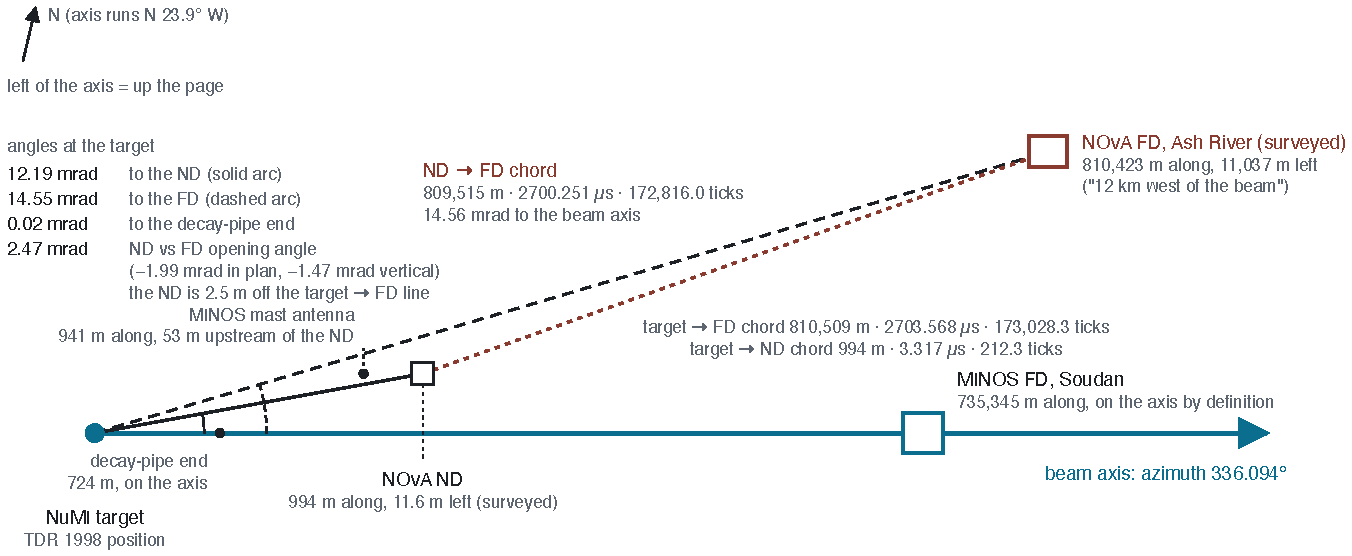
\includegraphics[width=\textwidth]{01-plan-view}
\caption{Plan view, not to scale: the beam axis from the NuMI target through the MINOS far detector, the surveyed \ND{} and \FD{} faces to its left, the MINOS mast antenna, and the chords used in the calculation.}
\label{fig:plan}
\end{figure}
\begin{figure}[htbp]\centering
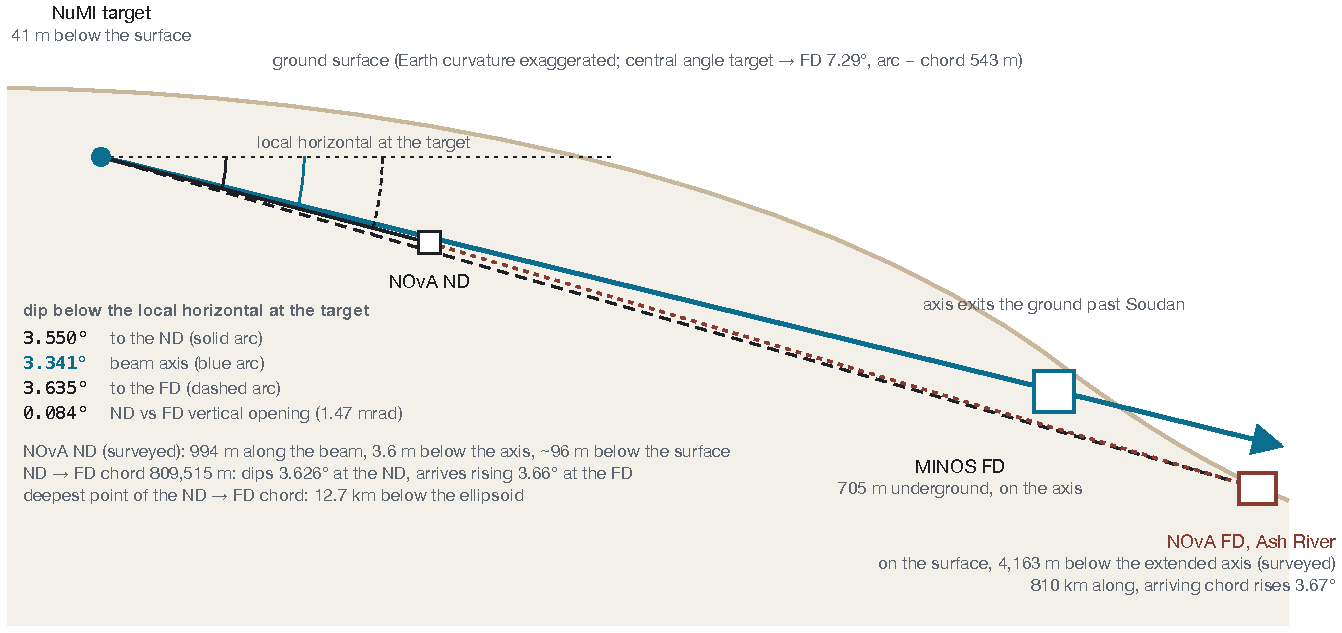
\includegraphics[width=\textwidth]{02-elevation-view}
\caption{Elevation view, not to scale: dips of the chords below the target's local horizontal, the curved ground surface, and the positions of the detectors relative to the extended beam axis.}
\label{fig:elev}
\end{figure}
\begin{figure}[htbp]\centering
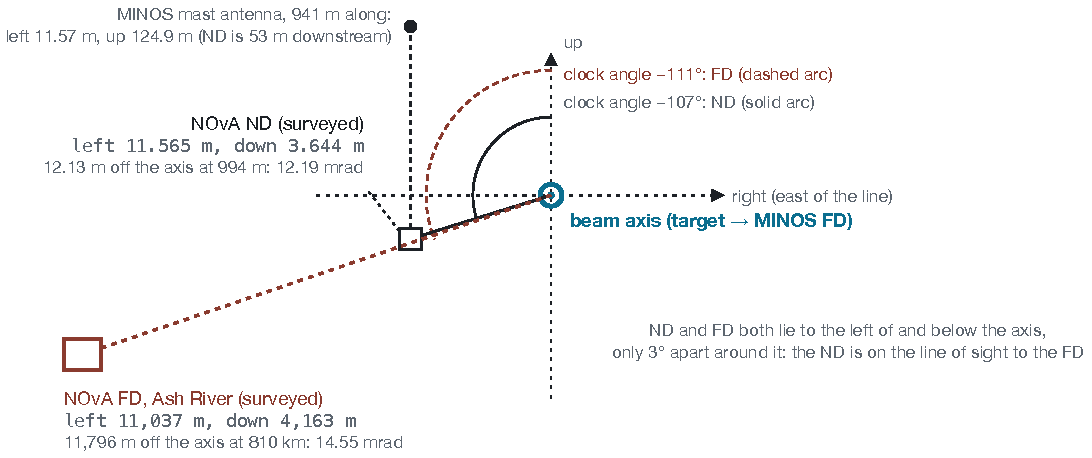
\includegraphics[width=0.85\textwidth]{03-transverse-view}
\caption{Transverse view looking downstream along the beam axis: the surveyed \ND{} and \FD{} faces lie to the left of and below the axis at almost the same clock angle.}
\label{fig:transverse}
\end{figure}

\section{Time of flight and timing offsets}
\subsection{Flight time and clock ticks}
With $c=\SI{299792458}{m/s}$ exactly and neutrinos taken to travel at $c$ (the mass-induced delay is evaluated in Sec.~\ref{sec:effects}),
\begin{equation}
t=\frac{L}{c},\qquad n=f_{\rm clk}\,t,\qquad f_{\rm clk}=\SI{64}{MHz},
\end{equation}
so one tick is \SI{15.625}{ns} or \SI{4.684}{m} of light path.  The legacy Global Trigger unit of \SI{500}{ns} is also given.  Table~\ref{tab:timing} lists the results for the surveyed geometry; the integer tick count uses round-to-nearest and the residual is the difference between the integer and the exact value.

\begin{table}[htbp]\centering\scriptsize
\caption{Flight times for the surveyed geometry.  ``total'' includes the Main Injector shift of Sec.~\ref{sec:mi}.}
\label{tab:timing}
\resizebox{\textwidth}{!}{\begin{tabular}{p{5.2cm}rrrrrrr}
\toprule
chord & $L$ (m) & $t$ (\textmu{}s) & ticks & integer & residual (ns) & 500 ns units & total ticks \\
\midrule
ND upstream face $\rightarrow$ FD upstream face (both surveyed) & \num{809514.750} & \num{2700.250552} & \num{172816.035} & \num{172816} & \num{-0.55} & \num{5400.5011} & \num{272736.417} \\
NuMI target $\rightarrow$ FD upstream face (surveyed) & \num{810509.171} & \num{2703.567584} & \num{173028.325} & \num{173028} & \num{-5.08} & \num{5407.1352} & \num{272948.707} \\
NuMI target $\rightarrow$ ND upstream face (surveyed) & \num{994.424} & \num{3.317043} & \num{212.291} & \num{212} & \num{-4.54} & \num{6.6341} & \num{100132.672} \\
MCZERO $\rightarrow$ FD upstream face (surveyed; stationing 810,422.324 m) & \num{810508.171} & \num{2703.564248} & \num{173028.112} & \num{173028} & \num{-1.75} & \num{5407.1285} & \num{272948.494} \\
MCZERO $\rightarrow$ ND upstream face (surveyed; stationing 993.350 m) & \num{993.424} & \num{3.313707} & \num{212.077} & \num{212} & \num{-1.21} & \num{6.6274} & \num{100132.459} \\
NuMI target $\rightarrow$ Lake Vermilion (-100 ft) & \num{739881.733} & \num{2467.979809} & \num{157950.708} & \num{157951} & \num{+4.57} & \num{4935.9596} & \num{257871.089} \\
ND upstream face $\rightarrow$ Lake Vermilion (-100 ft) & \num{738887.353} & \num{2464.662914} & \num{157738.426} & \num{157738} & \num{-6.66} & \num{4929.3258} & \num{257658.808} \\
NuMI target $\rightarrow$ Lake Superior, Two Harbors (-100 ft) & \num{633442.910} & \num{2112.938110} & \num{135228.039} & \num{135228} & \num{-0.61} & \num{4225.8762} & \num{235148.421} \\
ND upstream face $\rightarrow$ Lake Superior, Two Harbors (-100 ft) & \num{632448.627} & \num{2109.621539} & \num{135015.779} & \num{135016} & \num{+3.46} & \num{4219.2431} & \num{234936.160} \\
\bottomrule

\end{tabular}}
\end{table}

\subsection{Main Injector timing shift}
\label{sec:mi}
After the 2012 shutdown the beam moved relative to the Main Injector Beam Sync event MIBS\,\$74 by 141 MI revolutions \cite{norman2013nb}.  With $h_{\rm MI}=588$ RF buckets per turn at the flat-top RF frequency $f_{\rm RF}$,
\begin{equation}
T_{\rm rev}=\frac{h_{\rm MI}}{f_{\rm RF}},\qquad \Delta t_{\rm MI}=141\,T_{\rm rev},\qquad n_{\rm MI}=f_{\rm clk}\,\Delta t_{\rm MI},
\end{equation}
giving Table~\ref{tab:mi}.  One revolution is \num{708.655} ticks: the \SI{53.1034}{MHz} RF and the \SI{64}{MHz} clock are not commensurate, and a \SI{1}{kHz} error in $f_{\rm RF}$ shifts $n_{\rm MI}$ by \num{1.882}
ticks.

\begin{table}[htbp]\centering\small
\caption{Main Injector 141-turn shift.}
\label{tab:mi}
\begin{tabular}{rrrrrrr}
\toprule
turns & buckets/turn & $f_{\rm RF}$ (MHz) & $T_{\rm rev}$ (\textmu{}s) & ticks/turn & $\Delta t_{\rm MI}$ (\textmu{}s) & $n_{\rm MI}$ (ticks) \\
\midrule
\num{141} & \num{588} & \num{53.1034} & \num{11.072737} & \num{708.655} & \num{1561.255965} & \num{99920.382}
 \\
\bottomrule
\end{tabular}
\end{table}

\subsection{Combined offset and trigger window}
The total offset of the \FD{} trigger relative to MIBS\,\$74 is $n_{\rm tot}=n_{\rm ToF}+n_{\rm MI}$ (Table~\ref{tab:total}); the Sagnac term is reported but not added.  The window of Eq.~\eqref{eq:window} in ticks is given in Table~\ref{tab:window}; a \SI{50}{\micro s} window spans \num{3200} ticks and overlaps one or two \SI{50}{\micro s} microslices, so a recorded beam event is up to \SI{100}{\micro s} wide.

\begin{table}[htbp]\centering\small
\caption{Combined offset, \ND{} face $\to$ \FD{} face plus the MI shift.}
\label{tab:total}
\begin{tabular}{rrrrr}
\toprule
$n_{\rm ToF}$ & $n_{\rm MI}$ & $n_{\rm tot}$ & integer & residual (ns) \\
\midrule
\num{172816.035} & \num{99920.382} & \num{272736.417} & \num{272736} & \num{-6.52}
 \\
\bottomrule
\end{tabular}
\end{table}
\begin{table}[htbp]\centering\small
\caption{Trigger window $[t-\SI{20}{\micro s},\,t+\SI{30}{\micro s})$ in ticks after $t_0$, relative to the flight time alone and to the flight time plus the MI shift.}
\label{tab:window}
\resizebox{\textwidth}{!}{\begin{tabular}{rrrrrc}
\toprule
ToF low & ToF high & total low & total high & ticks/microslice & microslices overlapped \\
\midrule
\num{171536.04} & \num{174736.04} & \num{271456.42} & \num{274656.42} & \num{3200} & 1--2
 \\
\bottomrule
\end{tabular}}
\end{table}

\subsection{Effects outside the geometric flight time}
\label{sec:effects}
In the rotating ECEF frame a signal from $A$ to $B$ acquires the Sagnac correction $\Delta t_{\rm S}=\omega_\oplus\,(x_Ay_B-y_Ax_B)/c^2$ with $\omega_\oplus=\SI{7.2921150e-5}{rad/s}$ \cite{iers2010}; it is negative here because the beam travels westward and the \FD{} rotates toward it.  A neutrino of mass $m$ and energy $E$ is delayed by $\delta t=t\,m^2/(2E^2)$.  Antenna cable delays ($\ell/(v_f c)$) are receiver calibrations and not part of the flight time.  Table~\ref{tab:effects} lists them; the MINOS neutrino-speed measurement \cite{minostof2015} treats the same terms.

\begin{table}[htbp]\centering\small
\caption{Non-geometric terms for the \ND{} $\to$ \FD{} chord.}
\label{tab:effects}
\begin{tabular}{p{7.4cm}rrp{3.6cm}}
\toprule
effect & ns & ticks & status \\
\midrule
Sagnac (Earth rotation, ECEF frame) & \num{-1.303} & \num{-0.0834} & reported, not applied \\
neutrino mass delay ($m=\SI{0.1}{eV}$, $E=\SI{2}{GeV}$) & \num{3.38e-15} & \num{2.16e-16} & negligible \\
antenna cable delay, NOvA ND upstream face centre (Fermilab alignment survey) & \num{119.61} & \num{7.655} & receiver calibration, not ToF \\
antenna cable delay, NOvA FD upstream face centre (Fermilab alignment survey) & \num{119.61} & \num{7.655} & receiver calibration, not ToF \\
\bottomrule

\end{tabular}
\end{table}

\section{Angles relative to the beamline}
\subsection{Beam axis and off-axis positions}
The beam axis of this note is the line from the target through the MINOS \FD{} midpoint (Table~\ref{tab:axis}); the TDR design axis agrees with it in direction to \SI{0.02}{mrad}.  Table~\ref{tab:vsaxis} gives every site's off-axis angle at the target, distance along the axis and transverse position from Eq.~\eqref{eq:offaxis}.

\begin{table}[htbp]\centering\small
\caption{The beam axis.}
\label{tab:axis}
\resizebox{\textwidth}{!}{\begin{tabular}{lrrrl}
\toprule
axis & length (m) & azimuth at origin (\textdegree) & elevation at origin (\textdegree) & unit vector (ECEF) \\
\midrule
NuMI beam axis (target $\rightarrow$ MINOS FD) & \num{735344.614} & \num{336.09421} & \num{-3.34056} & (-0.424097927, 0.639571229, 0.641162687) \\
\bottomrule

\end{tabular}}
\end{table}

\begin{table}[htbp]\centering\small
\caption{Sites relative to the beam axis: off-axis angle at the target, distance along the axis, transverse distance with right/up components, and clock angle (\ang{0} above, \ang{90} right).}
\label{tab:vsaxis}
\resizebox{\textwidth}{!}{\begin{tabular}{lrrrrrr}
\toprule
id & off-axis (mrad) & along (m) & transverse (m) & right (m) & up (m) & clock (\textdegree) \\
\midrule
target & \num{0.0000} & \num{0.000} & \num{0.000} & \num{+0.000} & \num{+0.000} & -- \\
mczero & \num{0.1459} & \num{1.000} & \num{0.000} & \num{+0.000} & \num{+0.000} & \num{64.88} \\
decay-end & \num{0.0197} & \num{724.184} & \num{0.014} & \num{-0.000} & \num{+0.014} & \num{-1.89} \\
nd & \num{12.1935} & \num{994.350} & \num{12.125} & \num{-11.565} & \num{-3.643} & \num{-107.49} \\
fd & \num{14.5547} & \num{810423.324} & \num{11796.315} & \num{-11037.456} & \num{-4162.644} & \num{-110.66} \\
minos-fd & \num{0.0000} & \num{735344.614} & \num{0.000} & \num{+0.000} & \num{+0.000} & -- \\
nd-1015 & \num{12.4658} & \num{1015.000} & \num{12.653} & \num{-11.570} & \num{+5.123} & \num{-66.12} \\
nd-under-mast & \num{13.3426} & \num{948.316} & \num{12.654} & \num{-11.570} & \num{+5.123} & \num{-66.12} \\
fd2 & \num{14.5753} & \num{810478.514} & \num{11813.783} & \num{-11051.360} & \num{-4175.273} & \num{-110.70} \\
fnal-mast & \num{132.4921} & \num{941.341} & \num{125.455} & \num{-11.570} & \num{+124.921} & \num{-5.29} \\
\bottomrule

\end{tabular}}
\end{table}

The two lake sites fall close to the beam: Lake Vermilion lies \SI{740}{km} along the axis, \SI{2.3}{km} to its left and \SI{0.34}{km} above the extended axis line (\SI{3.17}{mrad} off axis), and the Two Harbors point lies almost exactly in the vertical plane of the axis (\SI{19}{m} to the right) \SI{633}{km} along it and \SI{5.4}{km} above the extended line (\SI{8.51}{mrad} off axis, clock angle \ang{0.2}, i.e.\ directly above the beam).

\subsection{Opening angles}
Table~\ref{tab:opening} gives the opening angles at the target between pairs of chords, their horizontal and vertical components, the transverse distance of the first endpoint from the second chord, and each chord's angle to the beam axis.  With both surveyed faces the \ND{} lies only \SI{2.46}{m} off the target $\to$ \FD{} line: the Near Detector sits on the line of sight to the Far Detector.

\begin{table}[htbp]\centering\scriptsize
\caption{Opening angles at the NuMI target.}
\label{tab:opening}
\resizebox{\textwidth}{!}{\begin{tabular}{p{5.6cm}rrrrrr}
\toprule
angle & total (mrad) & horizontal (mrad) & vertical (mrad) & $a$ transverse to $Vb$ (m) & $a$ vs axis (mrad) & $b$ vs axis (mrad) \\
\midrule
Target: ND vs FD (both surveyed) & \num{2.4740} & \num{-1.9895} & \num{-1.4705} & \num{2.460} & \num{12.1935} & \num{14.5547} \\
Target: ND (surveyed) vs MINOS FD & \num{12.1935} & \num{+11.6313} & \num{+3.6600} & \num{12.125} & \num{12.1935} & \num{0.0000} \\
Target: ND at the quoted 1015 m vs surveyed ND & \num{8.7139} & \num{-0.2374} & \num{-8.7107} & \num{8.845} & \num{12.4658} & \num{12.1935} \\
Target: ND under the mast (2014 note) vs surveyed ND & \num{9.0840} & \num{+0.5638} & \num{-9.0665} & \num{8.615} & \num{13.3426} & \num{12.1935} \\
Target: FD from the Ant-2 fix vs surveyed FD & \num{0.0223} & \num{+0.0162} & \num{+0.0152} & \num{18.037} & \num{14.5753} & \num{14.5547} \\
Target: ND vs Lake Vermilion & \num{9.4386} & \num{+8.4915} & \num{+4.1208} & \num{9.386} & \num{12.1935} & \num{3.1739} \\
Target: ND vs Lake Superior (Two Harbors) & \num{16.8551} & \num{+11.6647} & \num{+12.1668} & \num{16.760} & \num{12.1935} & \num{8.5068} \\
\bottomrule

\end{tabular}}
\end{table}

\subsection{Near Detector face edges}
The \ND{} face is \SI{158.125}{in} square (half-width \SI{2.0081875}{m}).  Table~\ref{tab:facend} gives the positions of its centre and edges and their angles to the beam axis; the face subtends \num{4.0386} mrad (left--right) and \num{4.0389} mrad (top--bottom)
 at the target.  Table~\ref{tab:facendfd} gives the opening angle between each face point and the target $\to$ \FD{} chord.  Figure~\ref{fig:face} shows the face with the iso-angle contours.  The \FD{} face (half-size \SI{304.21}{in}) is treated identically; its edges are \SI{0.019}{mrad} apart as seen from the target.

\begin{table}[htbp]\centering\scriptsize
\caption{\ND{} face points: geodetic position, angle to the beam axis and transverse offsets from the axis.}
\label{tab:facend}
\resizebox{\textwidth}{!}{\begin{tabular}{llllrrrr}
\toprule
point & latitude & longitude & $h$ (m) & angle to axis (mrad) & right (m) & up (m) & clock (\textdegree) \\
\midrule
left & 41\textdegree{} 50' 24.3203" N & 88\textdegree{} 16' 13.8777" W & \num{96.572} & \num{14.1325} & \num{-13.573} & \num{-3.643} & \num{-105.03} \\
center & 41\textdegree{} 50' 24.3467" N & 88\textdegree{} 16' 13.7981" W & \num{96.572} & \num{12.1935} & \num{-11.565} & \num{-3.643} & \num{-107.49} \\
right & 41\textdegree{} 50' 24.3731" N & 88\textdegree{} 16' 13.7185" W & \num{96.572} & \num{10.2854} & \num{-9.557} & \num{-3.643} & \num{-110.87} \\
top & 41\textdegree{} 50' 24.3501" N & 88\textdegree{} 16' 13.8002" W & \num{98.577} & \num{11.7457} & \num{-11.565} & \num{-1.635} & \num{-98.05} \\
bottom & 41\textdegree{} 50' 24.3432" N & 88\textdegree{} 16' 13.7961" W & \num{94.568} & \num{12.9444} & \num{-11.565} & \num{-5.652} & \num{-116.04} \\
\bottomrule

\end{tabular}}
\end{table}
\begin{table}[htbp]\centering\small
\caption{Opening angle at the target between each \ND{} face point and the chord to the \FD{} face.}
\label{tab:facendfd}
\resizebox{\textwidth}{!}{\begin{tabular}{lrrrrr}
\toprule
point & opening angle (mrad) & horizontal (mrad) & vertical (mrad) & transverse to the \FD{} chord (m) & chord vs axis (mrad) \\
\midrule
left & \num{1.4724} & \num{+0.0296} & \num{-1.4721} & \num{1.464} & \num{14.1325} \\
center & \num{2.4740} & \num{-1.9895} & \num{-1.4705} & \num{2.460} & \num{12.1935} \\
right & \num{4.2695} & \num{-4.0088} & \num{-1.4691} & \num{4.246} & \num{10.2854} \\
top & \num{4.0179} & \num{-1.9910} & \num{-3.4899} & \num{3.995} & \num{11.7457} \\
bottom & \num{2.0624} & \num{-1.9880} & \num{+0.5489} & \num{2.051} & \num{12.9444} \\
\bottomrule

\end{tabular}}
\end{table}

\begin{figure}[htbp]\centering
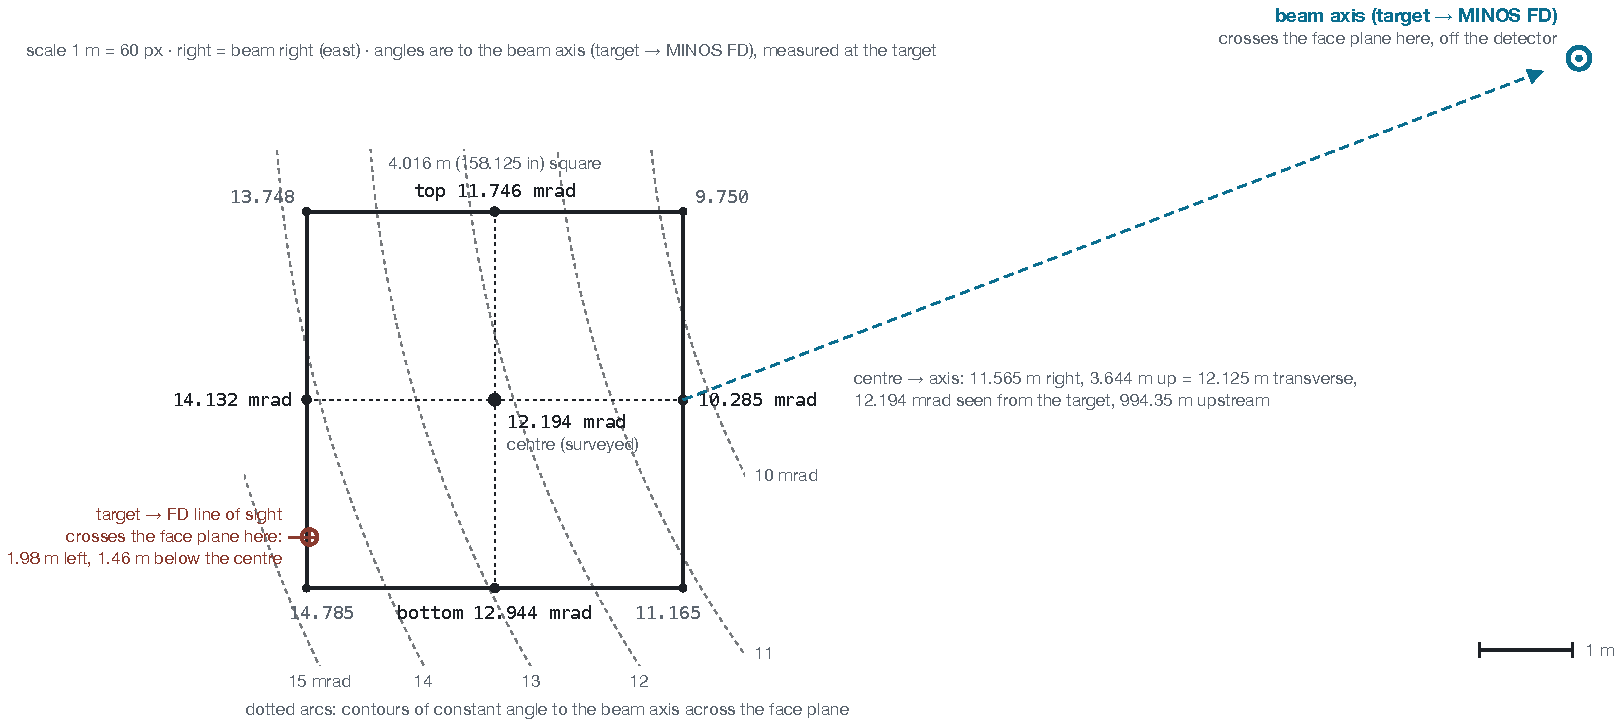
\includegraphics[width=\textwidth]{04-near-detector-front-face}
\caption{The \ND{} front face looking downstream, to scale: the angle to the beam axis at the centre, edges and corners, contours of constant angle across the face plane, the point where the beam axis crosses the face plane (off the detector, to the right and above), and the point where the target $\to$ \FD{} line of sight crosses the face plane.}
\label{fig:face}
\end{figure}

\section{Validation}
\label{sec:validation}
The target position and the realisation of the beamline frame rest on design documents; Table~\ref{tab:validation} checks them against independently published or surveyed quantities.  The target $\to$ MINOS \FD{} chord agrees with the published \SI{735338.0}{m} (from the horn-1 upstream end) to \SI{7}{m}, the beam azimuth with the 1999 geodetic survey to \ang{;;13}, the \FD{} ellipsoidal height with the NAVD88 survey elevation to \SI{0.3}{m} when the GEOID18 separation at Ash River (\SI{-31.221}{m}) is used (\SI{1.5}{m} with the receiver's own \SI{-32.462}{m}), and the MCZERO $\to$ \FD{} chord equals $\sqrt{X^2+Y^2+Z^2}$ of the survey coordinates identically.  The surveyed \ND{} confirms the 2014 antenna's \SI{11.57}{m} left offset to \SI{5}{mm}.  In addition the 2013 notebook is reproduced to $10^{-9}$ (Appendix~\ref{app:history}).

\begin{table}[htbp]\centering\small
\caption{Validation against published and surveyed quantities.}
\label{tab:validation}
\resizebox{\textwidth}{!}{\begin{tabular}{p{5.2cm}p{3cm}p{5cm}r}
\toprule
quantity & this note & reference & difference \\
\midrule
target $\rightarrow$ MINOS FD midpoint & \num{735344.6} m & \num{735338.0} m from horn 1 \citep{minos2008} & \num{+6.6} m \\
beam azimuth at the target & \num{336.09421}\textdegree{} & 336.09788\textdegree{} \citep{bocean1999} & \num{-0.00367}\textdegree{} \\
beam dip at the target & \num{3.34056}\textdegree{} & 3.34349\textdegree{} \citep{numibeam2016} & \num{-0.00293}\textdegree{} \\
decay-pipe length (TDR stations) & \num{675.0} m & 675 m \citep{numibeam2016} & -- \\
FD ellipsoidal height from the survey frame & \num{337.611} m & $H + N = 368.535 - 32.462 = 336.073$ m & \num{+1.54} m \\
MCZERO $\rightarrow$ FD chord vs $|(X,Y,Z)|$ & \num{810508.1714} m & \num{810508.1714} m & \num{+0.000000} m \\
off-axis angle of the FD face & \num{14.555} mrad & 14.6 mrad \citep{novasurvey} & -- \\
\bottomrule

\end{tabular}}
\end{table}

\section{Sensitivities and error budget}
Numerical partial derivatives of the \ND{} $\to$ \FD{} chord with respect to each input are given in Table~\ref{tab:sens}; the gradient of $L$ with respect to an endpoint position is the unit chord vector, so an endpoint error of $\sigma$ metres along the chord is worth $\sigma$ metres of $L$ (\SI{3.34}{ns/m}).  The error budget (Table~\ref{tab:budget}) combines the declared $1\sigma$ uncertainties in quadrature and lists conventions and neglected terms separately.  With both faces surveyed, the budget is dominated by the RF-frequency term of the Main Injector shift; combined items: root-sum-square \num{1.906} ticks (\num{29.8} ns), linear sum \num{2.309} ticks (\num{36.1} ns)
.

\begin{table}[htbp]\centering\scriptsize
\caption{Sensitivities of the \ND{} $\to$ \FD{} chord.}
\label{tab:sens}
\resizebox{\textwidth}{!}{\begin{tabular}{p{7.5cm}rrr}
\toprule
variation & $\Delta L$ (m) & $\Delta t$ (ns) & $\Delta$ticks \\
\midrule
NOvA ND upstream face centre (Fermilab alignment survey): height +1 m & \num{+0.0632} & \num{+0.211} & \num{+0.0135} \\
NOvA ND upstream face centre (Fermilab alignment survey): latitude +1" & \num{-27.9763} & \num{-93.319} & \num{-5.9724} \\
NOvA ND upstream face centre (Fermilab alignment survey): longitude +1" & \num{+9.6187} & \num{+32.085} & \num{+2.0534} \\
NOvA ND upstream face centre (Fermilab alignment survey): endpoint +1 m East & \num{+0.4169} & \num{+1.391} & \num{+0.0890} \\
NOvA ND upstream face centre (Fermilab alignment survey): endpoint +1 m North & \num{-0.9068} & \num{-3.025} & \num{-0.1936} \\
NOvA FD upstream face centre (Fermilab alignment survey): height +1 m & \num{+0.0638} & \num{+0.213} & \num{+0.0136} \\
NOvA FD upstream face centre (Fermilab alignment survey): latitude +1" & \num{+27.2369} & \num{+90.852} & \num{+5.8146} \\
NOvA FD upstream face centre (Fermilab alignment survey): longitude +1" & \num{-9.6182} & \num{-32.083} & \num{-2.0533} \\
NOvA FD upstream face centre (Fermilab alignment survey): endpoint +1 m East & \num{-0.4674} & \num{-1.559} & \num{-0.0998} \\
NOvA FD upstream face centre (Fermilab alignment survey): endpoint +1 m North & \num{+0.8817} & \num{+2.941} & \num{+0.1882} \\
spherical Earth (R = 6378137 m) at the final endpoints & \num{+822.9838} & \num{+2745.178} & \num{+175.6914} \\
GRS80 ellipsoid instead of WGS84 & \num{-0.0000} & \num{-0.000} & \num{-0.0000} \\
\bottomrule

\end{tabular}}
\end{table}
\begin{table}[htbp]\centering\small
\caption{Error budget, \ND{} face $\to$ \FD{} face, in \SI{64}{MHz} ticks.}
\label{tab:budget}
\resizebox{\textwidth}{!}{\begin{tabular}{p{7cm}rrll}
\toprule
source & ns & ticks & type & combined \\
\midrule
NOvA ND upstream face centre (Fermilab alignment survey): endpoint offset $\pm$1 m, worst case along the chord & \num{3.34} & \num{0.213} & systematic & yes \\
NOvA FD upstream face centre (Fermilab alignment survey): endpoint offset $\pm$1 m, worst case along the chord & \num{3.34} & \num{0.213} & systematic & yes \\
Main Injector 141-turn shift (2012 shutdown): RF frequency $\pm$1000 Hz & \num{29.40} & \num{1.882} & systematic & yes \\
integer rounding of the final tick count & \num{7.81} & \num{0.500} & convention & no \\
Sagnac term (not applied) & \num{1.30} & \num{0.083} & neglected & no \\
\bottomrule

\end{tabular}}
\end{table}

\section{Summary}
Table~\ref{tab:baselines} collects all baselines.  For the surveyed \ND{} and \FD{} faces the flight path is \SI{809514.750}{m}, the flight time \SI{2700.250552}{\micro s} = \num{172816.035} ticks, and the total offset with the 141-turn Main Injector shift \num{272736.417} ticks, i.e.\ \num{272736} ticks when rounded (residual \SI{-6.5}{ns}).  From the target the \FD{} face is \SI{810509.171}{m} (\num{173028.325} ticks) and the \ND{} face \SI{994.424}{m} (\num{212.291} ticks).  The \ND{} and \FD{} are \num{12.19} and \num{14.55}~mrad off the Soudan axis, on the same side (clock \ang{-107} and \ang{-111}), and the \ND{} face spans \num{4.04}~mrad at the target.  Chords from the target to the lake points are \SI{739881.733}{m} (Lake Vermilion, \num{157950.708} ticks) and \SI{633442.910}{m} (Two Harbors, \num{135228.039} ticks).  Open items are the as-built MCZERO and target positions (about \SI{1}{m} along the beam) and the lake-level datums.

\begin{table}[htbp]\centering\scriptsize
\caption{All baselines of the configuration.  ``total'' adds the MI shift; the last column is the opening angle between the chord and the beam axis.}
\label{tab:baselines}
\resizebox{\textwidth}{!}{\begin{tabular}{p{6.2cm}rrrrrr}
\toprule
baseline & $L$ (m) & $t$ (\textmu{}s) & ticks & total ticks & integer & chord vs axis (mrad) \\
\midrule
ND upstream face $\rightarrow$ FD upstream face (both surveyed) & \num{809514.750} & \num{2700.250552} & \num{172816.035} & \num{272736.417} & \num{272736} & \num{14.5576} \\
NuMI target $\rightarrow$ FD upstream face (surveyed) & \num{810509.171} & \num{2703.567584} & \num{173028.325} & \num{272948.707} & \num{272949} & \num{14.5547} \\
NuMI target $\rightarrow$ ND upstream face (surveyed) & \num{994.424} & \num{3.317043} & \num{212.291} & \num{100132.672} & \num{100133} & \num{12.1935} \\
MCZERO $\rightarrow$ FD upstream face (surveyed; stationing 810,422.324 m) & \num{810508.171} & \num{2703.564248} & \num{173028.112} & \num{272948.494} & \num{272948} & \num{14.5547} \\
MCZERO $\rightarrow$ ND upstream face (surveyed; stationing 993.350 m) & \num{993.424} & \num{3.313707} & \num{212.077} & \num{100132.459} & \num{100132} & \num{12.2059} \\
ND at the quoted 1015 m $\rightarrow$ FD (superseded ND placement) & \num{809494.148} & \num{2700.181830} & \num{172811.637} & \num{272732.019} & \num{272732} & \num{14.5618} \\
ND under the mast $\rightarrow$ FD from the Ant-2 fix (superseded 2014-note geometry) & \num{809616.263} & \num{2700.589164} & \num{172837.706} & \num{272758.088} & \num{272758} & \num{14.5812} \\
NuMI target $\rightarrow$ Lake Vermilion (-100 ft) & \num{739881.733} & \num{2467.979809} & \num{157950.708} & \num{257871.089} & \num{257871} & \num{3.1739} \\
ND upstream face $\rightarrow$ Lake Vermilion (-100 ft) & \num{738887.353} & \num{2464.662914} & \num{157738.426} & \num{257658.808} & \num{257659} & \num{3.1634} \\
NuMI target $\rightarrow$ Lake Superior, Two Harbors (-100 ft) & \num{633442.910} & \num{2112.938110} & \num{135228.039} & \num{235148.421} & \num{235148} & \num{8.5068} \\
ND upstream face $\rightarrow$ Lake Superior, Two Harbors (-100 ft) & \num{632448.627} & \num{2109.621539} & \num{135015.779} & \num{234936.160} & \num{234936} & \num{8.5261} \\
NuMI target $\rightarrow$ MINOS FD (validation of the target position) & \num{735344.614} & \num{2452.845607} & \num{156982.119} & \num{256902.501} & \num{256903} & \num{0.0000} \\
NuMI target $\rightarrow$ decay-pipe end (TDR design axis) & \num{724.184} & \num{2.415619} & \num{154.600} & \num{100074.981} & \num{100075} & \num{0.0197} \\
\bottomrule

\end{tabular}}
\end{table}

\appendix
\section{History and reproduction of the earlier calculations}
\label{app:history}
The 2013 notebook \cite{norman2013nb} used the MINOS mast antenna (\ang{41;50;23}\,N, \ang{88;16;13}\,W, \SI{228}{m}) lowered by \SI{300}{m} and Ash River antenna~2 (\SI{348.638}{m}); the 2014 note \cite{norman2014} specified $105+15$~m and $12+7.8$~m vertical offsets instead and left the horizontal antenna-to-detector vectors to be determined.  Table~\ref{tab:repro} reproduces the notebook's printed outputs with the present code, and Table~\ref{tab:ledger2014} shows the 2014-note ledger.  Table~\ref{tab:history} traces the \ND{} $\to$ \FD{} tick count through the successive geometries: the 2014 antenna-derived endpoints, the Near Detector placed at a quoted \SI{1015}{m} from the target with the antenna's transverse position, and the surveyed faces.  The surveyed \FD{} face is \SI{58}{m} horizontally and \SI{8.8}{m} vertically from the antenna-derived point; the surveyed \ND{} face is \SI{993.35}{m} from MCZERO, \SI{3.6}{m} below the axis, not \SI{5.1}{m} above it.

\begin{table}[htbp]\centering\small
\caption{Reproduction of the 2013 notebook \cite{norman2013nb}; the last row is the 2014-note offset geometry.}
\label{tab:repro}
\begin{tabular}{lrrr}
\toprule
quantity & recomputed & notebook & relative difference \\
\midrule
2013 notebook, spherical chord (m) & \num{810429.1726} & \num{810429.1726} & \num{7.2e-16} \\
2013 notebook, WGS84 chord (m) & \num{809606.1622} & \num{809606.1622} & \num{5.8e-16} \\
2013 notebook, ToF (\textmu{}s) & \num{2700.555470} & \num{2700.555470} & \num{6.7e-16} \\
2013 notebook, ToF (ticks) & \num{172835.5501} & \num{172835.5501} & \num{5.1e-16} \\
2013 notebook, MI shift (ticks) & \num{99920.3817} & \num{99920.3817} & \num{1.5e-16} \\
2013 notebook, total (ticks) & \num{272755.9318} & \num{272755.9318} & \num{2.1e-16} \\
2014 note offsets, WGS84 chord (m) & \num{809616.2634} & -- & -- \\
\bottomrule

\end{tabular}
\end{table}
\begin{table}[htbp]\centering\scriptsize
\caption{Correction ledger of the superseded 2014-note geometry (antenna fixes with vertical offsets).}
\label{tab:ledger2014}
\resizebox{\textwidth}{!}{\begin{tabular}{lp{6cm}rrrr}
\toprule
step & applied & $L$ (m) & $\Delta L$ (m) & $\Delta t$ (ns) & $\Delta$ticks \\
\midrule
reference model & spherical Earth, R = 6378137.000 m; heights as given; surveyed points, no offsets & \num{810448.173} & \num{+0.000} & \num{+0.00} & \num{+0.000} \\
Earth model & WGS84 ellipsoid; heights as given; surveyed points, no offsets & \num{809625.125} & \num{-823.048} & \num{-2745.39} & \num{-175.705} \\
vertical offset & ND endpoint if it were under the MINOS mast (105 + 15 m down): endpoint -120.000 m along the local geodetic vertical (105 m cavern depth + 15 m mast) & \num{809617.527} & \num{-7.598} & \num{-25.35} & \num{-1.622} \\
vertical offset & Ash River Ant-2 fix, front face via -19.8 m (antenna-derived, superseded): endpoint -19.800 m along the local geodetic vertical (12 m antenna $\rightarrow$ detector top + 7.8 m to mid-height) & \num{809616.263} & \num{-1.263} & \num{-4.21} & \num{-0.270} \\
\bottomrule

\end{tabular}}
\end{table}
\begin{table}[htbp]\centering\small
\caption{\ND{} $\to$ \FD{} tick count through the successive geometries.}
\label{tab:history}
\begin{tabular}{lrr}
\toprule
geometry & ticks & vs surveyed \\
\midrule
2013 notebook: antenna $-$300 m, no FD offset & \num{172835.550} & \num{+19.515} \\
2014 note: antenna $-$120 m, FD antenna $-$19.8 m & \num{172837.706} & \num{+21.671} \\
ND at the quoted 1015 m, antenna transverse & \num{172811.637} & \num{-4.398} \\
surveyed faces (this note) & \num{172816.035} & \num{+0.000} \\
\bottomrule

\end{tabular}
\end{table}

\section{Software and reproducibility}
All numbers were produced by \code{gps-tof} \cite{gpstof} (Python, standard library plus PyYAML) from the configuration \code{config/nova.yaml}, which records every input with its source.  The package implements Eqs.~\eqref{eq:ecef}--\eqref{eq:offaxis}, the correction ledger, the sensitivities and the error budget, and is covered by a test suite that pins the reproduction of the 2013 notebook, the EPSG worked example, the Beams-doc-1148 control points, the survey coordinates and the headline results.  To regenerate the report and this note's tables:
\begin{verbatim}
gps-tof -c config/nova.yaml -f all -o reports/nova
python3 scripts/make_note_tables.py
cd docs/note && latexmk -pdf nova-tof-note
\end{verbatim}
Local copies of every cited document are kept in \code{docs/external/} and \code{docs/reference/} of the repository, with SHA-256 checksums and an index of provenance.

\bibliographystyle{unsrtnat}
\bibliography{references}
\end{document}
